\documentclass[conference]{IEEEtran}
\IEEEoverridecommandlockouts
% The preceding line is only needed to identify funding in the first footnote. If that is unneeded, please comment it out.
\usepackage{cite}
\usepackage{amsmath,amssymb,amsfonts}
\usepackage{algorithmic}
\usepackage{graphicx}
\usepackage{textcomp}
\usepackage{xcolor}
\usepackage{tikz}
\usepackage{tabularx}
\usepackage{array}
\usepackage{makecell}
\usepackage{float}
\def\BibTeX{{\rm B\kern-.05em{\sc i\kern-.025em b}\kern-.08em
    T\kern-.1667em\lower.7ex\hbox{E}\kern-.125emX}}
\usetikzlibrary{shapes.geometric, arrows}
\newcolumntype{L}[1]{>{\raggedright\arraybackslash}p{#1}}

\tikzstyle{startstop} = [rectangle, rounded corners, minimum width=3cm, minimum height=1cm, text centered, draw=black, fill=red!30]
\tikzstyle{process} = [rectangle, minimum width=2.7cm, minimum height=1cm, text centered, draw=black, fill=orange!30]
\tikzstyle{decision} = [diamond, minimum width=3cm, minimum height=1cm, text centered, draw=black, fill=green!30]
\tikzstyle{arrow} = [thick,->,>=stealth]
\raggedbottom
\begin{document}

\title{A Proximal Policy Optimization Approach to Detect Spoofing in Algorithmic Trading}

\author{\IEEEauthorblockN{Iulia-Diana Groza}
\IEEEauthorblockA{\textit{Faculty of Mathematics and Computer Science} \\
\textit{Babes-Bolyai University}\\
Cluj-Napoca, Romania \\
iulia.groza@stud.ubbcluj.ro}
}

\maketitle

\begin{abstract}
Among the most pressing issues in algorithmic trading are spoofing tactics, where traders deceive other market participants by placing and then quickly canceling large orders. This leads to artificial price movements and compromises the trust in market fairness. This paper explores the development of a Proximal Policy Optimization agent to detect spoofing in real time using Level 3 Limit Order Book data from the LUNA flash crash in May 2022. We develop an anomaly detection system to label legitimate spoofing attempts. Ultimately, we simulate the market environment serving as the playground for our policy network. Our core contributions include the integration of Proximal Policy Optimization in market surveillance, the use of Level 3 Level Order Book data in a machine learning solution to harness temporal data, and the feature engineering of rolling statistics for price and size movements. Our experimental results demonstrate the feasibility of deep reinforcement learning in advancing market integrity.
\end{abstract}

\begin{IEEEkeywords}
proximal policy optimization, algorithmic trading, spoofing, deep reinforcement learning, anomaly detection
\end{IEEEkeywords}

\section{Introduction}
With the rise of algorithmic trading in recent decades, financial markets have been drastically transformed: significant efficiencies have appeared, but the major caveat that algorithmic trading introduced is its effect on market integrity \cite{Hendershott_Riordan_2013}. Among the most pressing issues are the manipulative practices of spoofing, where traders deceive other market participants by placing and then quickly canceling large orders. These tactics can lead to artificial price movements and compromise the trust in market fairness \cite{Armour_PFR}. Spoofing is an illegal practice governed by multiple laws in both the European Union and the United States, with the Dodd-Frank Act \cite{Dodd_Frank} being the most notable legal framework for market manipulation.

This paper explores the application of Proximal Policy Optimization (PPO), a deep reinforcement learning technique, to detect spoofing in algorithmic trading. We aim to develop a real-time detection system, integrated in a web application.

Our main motivation for this study is the lack of existing web-based tools for market manipulation detection that could help traders gain a better understanding of the current market situation and make informed decisions promptly before participating in the market. To the best of our knowledge, there is no web tool that allows online investors to analyze the status of market integrity in real time.

The core of this study involves the design and implementation of a PPO-based spoofing detection model. We utilize historical Level 3 Limit Order Book (LOB) data from the LUNA flash crash in May 2022, offering a realistic and challenging testbed for our approach. The data and statistical reports on order cancellation during that event have been procured from the work of Li, Polukarov, and Ventre (2023) \cite{Li_2023}. Since the LOB data is not labeled, we develop an anomaly detection system that allows us to effectively label legitimate spoofing attempts.

This model is integrated into a web application, \textit{spoof.io}, which provides a practical tool for monitoring trading activities and identifying spoofing in LUNA trades. Working as a proof-of-concept tool, the application will simulate the last two hours of the LUNA flash crash from May 2022, which represent our test data.

Ultimately, this work aims to contribute to the field of market surveillance in several ways. To the best of our knowledge, there is no work in the financial markets field that employs PPO in a market manipulation detector. Additionally, our approach advances the use of Level 3 LOB data in a machine learning solution to harness temporal data. To achieve this, we build on existing statistical physics methodologies, such as those by Li, Polukarov, and Ventre (2023) \cite{Li_2023}. Finally, our contribution brought during the anomaly detection phase includes the feature engineering of rolling statistics on order price and size, such as mean, standard deviation, and variance, which provide additional information on market volatility during the computation of the anomaly score.

\section{Related Work}
\par Supervised learning models, particularly those employing deep learning architectures like Gated Recurrent Units (GRU) and Feedforward Neural Networks (FNN), have shown high accuracy in detecting known patterns of market manipulation. The GRU-based model developed by Tuccella, Nadler, and Serban (2021) achieved an accuracy of 0.75 \cite{Tuc_2021}, which is commendable for real-time detection. However, these models require extensive labeled datasets for training, which can be a significant limitation in markets where manipulation tactics evolve rapidly.

\par On the other hand, the FNN model discussed by Leangarun, Tangamchit, and Thajchayapong (2016) \cite{Leang_2016} demonstrated the impact of data granularity by showing improved results with Level 2 data over Level 1 data, highlighting the importance of detailed order book information (especially on cancellation orders and their depth) in enhancing accuracy of manipulation detection \cite{Leang_2016}.

\par The Adaptive Hidden Markov Model with Anomaly States (AHMMAS) introduced by Cao, Li, Coleman, Belatreche, and McGinnity (2016) \cite{Cao_2015} represents a significant advancement in unsupervised detection methods. It outperformed traditional models by effectively recognizing anomalous trading patterns without prior labeling of L2 snapshots \cite{Cao_2015}. Although this model offers powerful detection capabilities and adapts to new data through its sliding window mechanism, its complexity and computational demands could pose challenges for real-time market surveillance.

\par The works of Lillo and Farmer (2005) \cite{Lillo_2005}, and Yura, Takayasu, Sornette, and Takayasu (2014) \cite{Yura_2014} provide foundational insights into how liquidity fluctuations and price movements can be analyzed using statistical physics. Their methods are particularly adept at capturing complex interactions within the order book that traditional models might overlook. This demonstrates the complex interplay between market orders, limit orders, and cancellations, a remark that is essential in our study conducted on spoofing.

\par Li, Polukarov, and Ventre's approach \cite{Li_2023} successfully applied these principles to detect spoofing \& layering during the LUNA cryptocurrency flash crash. Their model, which considers orders as particles whose interactions can be quantified and analyzed, showcased superior performance in identifying manipulative behaviors that were not detected by more traditional Z-score-based anomaly detection methods. Their work proved that the use of more granular data, of Level 3, can be both successful and computationally efficient at the same time.

\par When comparing all methods, it's evident that while supervised and unsupervised learning strategies provide accurate tools for detecting known and evolving manipulative patterns, statistical physics approaches bring a novel and profound analytical depth. An ideal solution would combine the simplicity and computational power of supervised learning in real-time detection, the absence of a requirement for labeled data in unsupervised learning strategies, and the accuracy given by state-of-the-art econophysics methods. We consider that a PPO-based approach will effectively harness most of these advantages.

\par In 2022, Chip Huyen presented in one of her most acclaimed pieces of work, \textit{Designing Machine Learning Systems}, a 2020 survey analyzing the large landscape of use cases of enterprise ML (in both internal and external scopes) \cite{Huyen_DMLS}. It points out that \textit{27\%} of enterprise ML applications focus on \textit{"Detecting fraud"}. This demonstrates the feasibility of utilizing ML techniques in our work in detecting forms of financial market manipulation such as spoofing.

\par Proven successful on a wide variety of tasks from robotic control to surpassing grandmasters at multiple strategy games, Proximal Policy Optimization (PPO) is a deep reinforcement learning algorithm designed by OpenAI in 2017. Since then, it became the default RL algorithm used by the AI research company, due to its simplicity and outstanding performance \cite{OpenAIPPO}.

\par PPO is a policy gradient method \cite{schulman2017proximal}. Therefore, unlike Deep-Q Network, it does not rely on experience replay (where transition experiences are stored in a replay buffer \cite{roderick2017implementing}); instead the agent learns online. The method has been introduced by Schulman, Levine, Abbeel, Jordan, and Moritz (2017) \cite{schulman2017proximal}, with Trust Region Policy Optimization serving as the foundational algorithm on which it has been built two years earlier by the same authors \cite{TRPO}.

\section{Data Collection and Feature Engineering}
\subsection{Collection and Preprocessing}
\par Spoofing frequently occurs in events marked by market instability, such as flash crashes \cite{Montgomery_SMMLOB}. Therefore, when collecting our data, we took several important aspects into consideration. Analyzing Level 3 (the most granular level) LOB data as part of a PPO-based detector is extremely important, as it marks our contribution and effectively leverages temporal data. Additionally, procuring data from recent flash crashes is essential as there are higher chances of subtle spoofing practices occurring in more recent data \cite{Kularatnam2024}. Finally, since we employ unsupervised methods, to ensure the correctness of our model evaluation, we must use historical data for which statistical reports on spoofing attempts were already performed, verified, and are publicly available. 

\par All these considerations led to our decision to work on the wLUNA/USD data utilized by Li, Polukarov, and Ventre (2023) \cite{Li_2023}. It was initially fetched from Coinbase via a WebSocket feed, and it consists of historical Level 3 LOB data on wLUNA/USD from the LUNA flash crash from May 2022 (11/05/2022, 16:00-20:00).

\par Orders placed at a price that matches or is less favorable than an existing order (typically the best bid or ask) are executed immediately, resulting in a $match$ record. Orders that are not executed or only partially executed become limit orders in the LOB, creating an $open$ record. These limit orders will remain in the LOB until they are canceled, generating a $canceled$ record. The minimum price precision is 0.01 USD, and the smallest trading volume unit (order size) is 0.001 LUNA. The timestamps are recorded with a precision of one microsecond, and are marked when an order activity (or event) occurs, making these event-driven timestamps discrete and non-consecutive \cite{Li_2023}.

\par The raw data consists of six JSON files: three for the full channel data and three for the ticker data. The event is split across three temporal windows (16:00 - 17:00, 18:00 - 19:00, respectively 19:00 - 20:00), each of the three files corresponding to one temporal window.

\par The first step in the preprocessing pipeline is to handle the temporal aspects of the data. We extract the hour of the day from each timestamp, as trading behaviors often exhibit diurnal patterns. By including the hour of the day as a feature, we allow the model to learn and leverage these temporal patterns, which can indicate spoofing activities that may occur at specific times.

\begin{table}[H]
    \centering
    \caption{Summary of raw dataset JSON files and their record counts}
    \label{table:json_files}
    \vspace{0.5cm}
    \begin{tabular}{|c|l|r|}
        \hline
        \textbf{\#} & \textbf{File Name} & \textbf{Number of Records} \\
        \hline
        1 & FullChannel\_GDAX\_20220511\_17hr.json & 768,272 \\
        \hline
        2 & FullChannel\_GDAX\_20220511\_19hr.json & 456,282 \\
        \hline
        3 & FullChannel\_GDAX\_20220511\_20hr.json & 550,124 \\
        \hline
         & \textbf{Total Full Channel Records} & \textbf{1,774,678} \\
        \hline
        4 & Ticker\_GDAX\_20220511\_17hr.json & 37,761 \\
        \hline
        5 & Ticker\_GDAX\_20220511\_19hr.json & 27,864 \\
        \hline
        6 & Ticker\_GDAX\_20220511\_20hr.json & 37,180 \\
        \hline
        & \textbf{Total Ticker Records} & \textbf{102,805} \\
        \hline
    \end{tabular}
\end{table}

\par Next, we address the issue of missing values, which is a common challenge in financial datasets. For numeric features, we employ median imputation to fill in missing values. The median is chosen for its ability to eliminate outliers, ensuring that the central tendency of the data is preserved. This step prevents the disruption of the model's learning process due to incomplete data.

\par Normalization is the next step in the preprocessing pipeline. By applying MinMaxScaler, we scale the numeric features to a range between 0 and 1. Consistent scaling facilitates faster convergence and improves the overall stability of the learning process. The normalization for a feature $x$ is given by:
\begin{equation}
x' = \frac{x - x_{\min}}{x_{\max} - x_{\min}}
\end{equation}

where $x_{\min}$ and $x_{\max}$ are the minimum and maximum values of the feature $x$, respectively.

\par Categorical features are processed through one-hot encoding, transforming them into binary vectors, therefore, each category is treated as a distinct entity without imposing any ordinal relationships. For instance, order types such as $received$, $open$, $done$, and $match$ are each represented as separate binary features. 

\par $remaining\_size\_change$ captures the dynamics of order size changes over time. By calculating the difference in remaining sizes across consecutive records grouped by order ID, we can identify patterns indicative of spoofing, such as frequent and abrupt changes in order sizes. This feature provides the model with additional insights into the aggressive placement and cancellation of orders. Formally, for an order $i$ with size $s$ at time $t$, the change in remaining size $\Delta s_i$ can be represented as:
\begin{equation}
\Delta s_i = s_i(t) - s_i(t-1)
\end{equation}

\par For the full channel data, we maintain identifiers such as $order\_id$ and $time$ to preserve traceability. The ticker data complements the order book data by providing additional context on price movements and trading volumes.

\subsection{Feature Engineering}
\par We mark our contribution by designing and processing features that effectively harness temporal data and financial statistics. Our objective is to fully leverage the theoretical foundations and spoofing preconditions outlined and applied by Leangarun, Tangamchit, and Thajchayapong (2016) \cite{Leang_2016}, while still introducing innovative and heuristic elements into our approach. 

\par We begin by calculating rolling statistics such as mean ($\mu$), standard deviation ($\sigma$), and variance ($\sigma^2$) for windows on multiple sizes (5, 10, and 15) on important columns like $price$ and $size$. These statistics provide us with a detailed view of the central tendency and dispersion of the data over different time periods. This allows us to identify abnormal fluctuations in price and order sizes, which are indicative of spoofing. A sudden increase in the variance of order sizes, for example, may suggest the presence of spoof orders intended to create a false impression of market depth.

\par Next, we compute the order flow imbalance (OFI), which measures the discrepancy between buy and sell orders over a rolling window. This is achieved by assigning a signed size to each order (positive for buy orders and negative for sell orders) and summing these sizes over the window. The OFI directly reflects market pressure, caused by the imbalance between buy and sell orders. Mathematically, the OFI can be expressed as:
\begin{equation}
OFI(t) = \sum_{i=t-w}^{t} size_i \cdot side_i
\end{equation}
where $w$ is the window size, $size_i$ is the size of order $i$, and $side_i$ is +1 for buy orders and -1 for sell orders. High positive or negative OFI values indicate significant market pressure, which can signal spoofing activities.

\par We also add the cancellation ratio to the dataset, which is the ratio of canceled orders to received orders. This ratio is a significant indicator of spoofing, as spoofers often place a large number of orders and cancel them quickly to create a misleading sense of market activity. The cancellation ratio (CR) is calculated as:
\begin{equation}
CR = \frac{reason\_canceled}{type\_received\_adjusted}
\end{equation}
where $type\_received\_adjusted$ ensures that the denominator is never zero by replacing zero values with one. A high cancellation ratio suggests a higher likelihood of spoofing.

\par The market spread is calculated as the difference between the best ask and best bid prices. The market spread ($spread$) provides insight into the market's liquidity and the aggressiveness of trading activities. It is expressed as:
\begin{equation}
spread = best\_ask - best\_bid
\end{equation}
A large spread often indicates uncertainty or manipulation in the market, which is commonly associated with spoofing.

\par Additionally, we one-hot encode the $hour\_of\_day$ feature to capture diurnal patterns in trading activity. This encoding ensures each hour is represented as a separate binary feature, allowing the model to identify time-specific spoofing behaviors.

\begin{figure}[H]
    \centering
    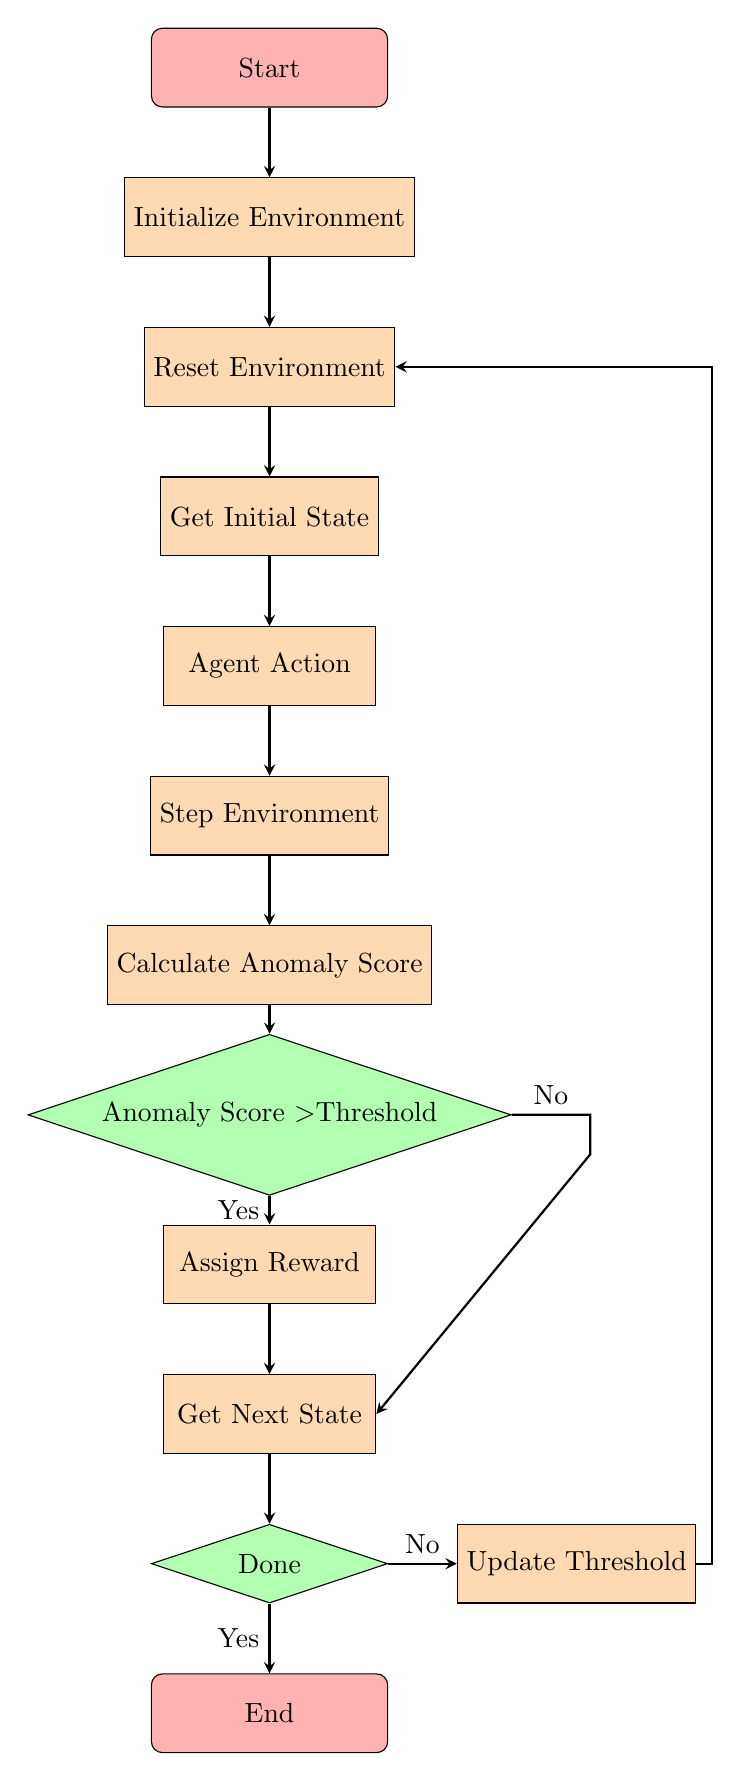
\begin{tikzpicture}[node distance=1.9cm]

        % Nodes
        \node (start) [startstop] {Start};
        \node (init) [process, below of=start] {Initialize Environment};
        \node (reset) [process, below of=init] {Reset Environment};
        \node (getstate) [process, below of=reset] {Get Initial State};
        \node (action) [process, below of=getstate] {Agent Action};
        \node (step) [process, below of=action] {Step Environment};
        \node (calcAnomaly) [process, below of=step] {Calculate Anomaly Score};
        \node (decision) [decision, below of=calcAnomaly, aspect=3] {Anomaly Score \textgreater Threshold};
        \node (reward) [process, below of=decision] {Assign Reward};
        \node (nextstate) [process, below of=reward] {Get Next State};
        \node (done) [decision, below of=nextstate, aspect=2.5] {Done};
        \node (update) [process, right of=done, xshift=2cm] {Update Threshold};
        \node (end) [startstop, below of=done] {End};
            
        % Arrows
        \draw [arrow] (start) -- (init);
        \draw [arrow] (init) -- (reset);
        \draw [arrow] (reset) -- (getstate);
        \draw [arrow] (getstate) -- (action);
        \draw [arrow] (action) -- (step);
        \draw [arrow] (step) -- (calcAnomaly);
        \draw [arrow] (calcAnomaly) -- (decision);
        \draw [arrow] (decision) -- node[anchor=east] {Yes} (reward);
        \draw [arrow] (reward) -- (nextstate);
        \draw [arrow] (nextstate) -- (done);
        \draw [arrow] (done) -- node[anchor=east] {Yes} (end);
        \draw [arrow] (done.east) -- node[anchor=south] {No} (update.west);
        \draw [arrow] (update.east) -- ++(0.2,0) |- (reset.east);
        \draw [arrow] (decision.east) -- node[anchor=south] {No} ++(1,0) |- ++(0,-0.5) -- (nextstate.east);
    \end{tikzpicture}
    \caption{Market Simulation Environment Pipeline}
    \label{fig:market_simulation_environment}
\end{figure}

\section{Proximal Policy Optimization Model}
\subsection{Market Simulation Environment}
\par The market simulation environment provides a controlled setting where the PPO model can interact with historical market data, learn patterns, and improve its detection capabilities.

\par The environment maintains \texttt{current\_index} to track the current position in the dataset, ensuring that the agent processes data sequentially. The  reset mechanism reinitializes the environment to its starting state, setting \texttt{current\_index} to a valid position within the data bounds and updating the spoofing threshold. This ensures that each training episode starts afresh, providing the model with a consistent and repeatable starting point.

\par The step processes the agent's actions, advances the market simulation by one step, and returns the new state, reward, and other relevant metrics. The reward structure is designed to reinforce correct detection of spoofing and penalize incorrect actions. This is mathematically represented as:
\begin{equation}
\begin{split}
reward = 
\begin{cases} 
1 & \text{if } (action = 1 \text{ and } is\_spoofing) \\
  & \text{or } (action = 0 \text{ and } \neg is\_spoofing), \\
-1 & \text{otherwise.}
\end{cases}
\end{split}
\end{equation}
where $is\_spoofing$ is determined by comparing the anomaly score to the spoofing threshold.

\par The state getter generates the current state by concatenating historical features from both full channel and ticker datasets. This approach ensures that the state includes a comprehensive view of market conditions over a specified history window.

\par Finally, since our dataset is not labeled, we need a method to assess the correctness of the agent's decisions and correlate it with the reward system. For this, we perform anomaly detection on orders. The anomaly score for each order is calculated based on predefined feature weights and market data features at the given index. The score is computed as:
\begin{equation}
anomaly\_score = \sum_{i} w_i \cdot \log(1 + |feature_i|)
\label{eq:anomaly_score}
\end{equation}

\par To adapt to changing market conditions, we implement an adaptive spoofing threshold that is dynamically updated based on recent anomaly scores. This ensures that the model remains responsive to shifts in market behavior. The threshold is updated to the $75\%$ of the recent anomaly scores, represented as:
\begin{equation}
\begin{split}
spoofing\_threshold = \text{percentile}(&\{anomaly\_score_i\}_{i=n-50}^{n}, \\
&75)
\end{split}
\end{equation}
where $n$ is the current index in the dataset.

\subsection{Policy Network}
\par The PPO Policy Network is implemented using PyTorch and features a straightforward FNN architecture. The network consists of an input layer with 690 neurons, two hidden layers with 256 neurons each, and an output layer. Each hidden layer employs ReLU activation functions to introduce non-linearity, allowing the network to capture complex patterns within the trading data. Additionally, the network uses a softmax activation function in the output layer to produce action probabilities.

\begin{figure}[H]
    \centering
    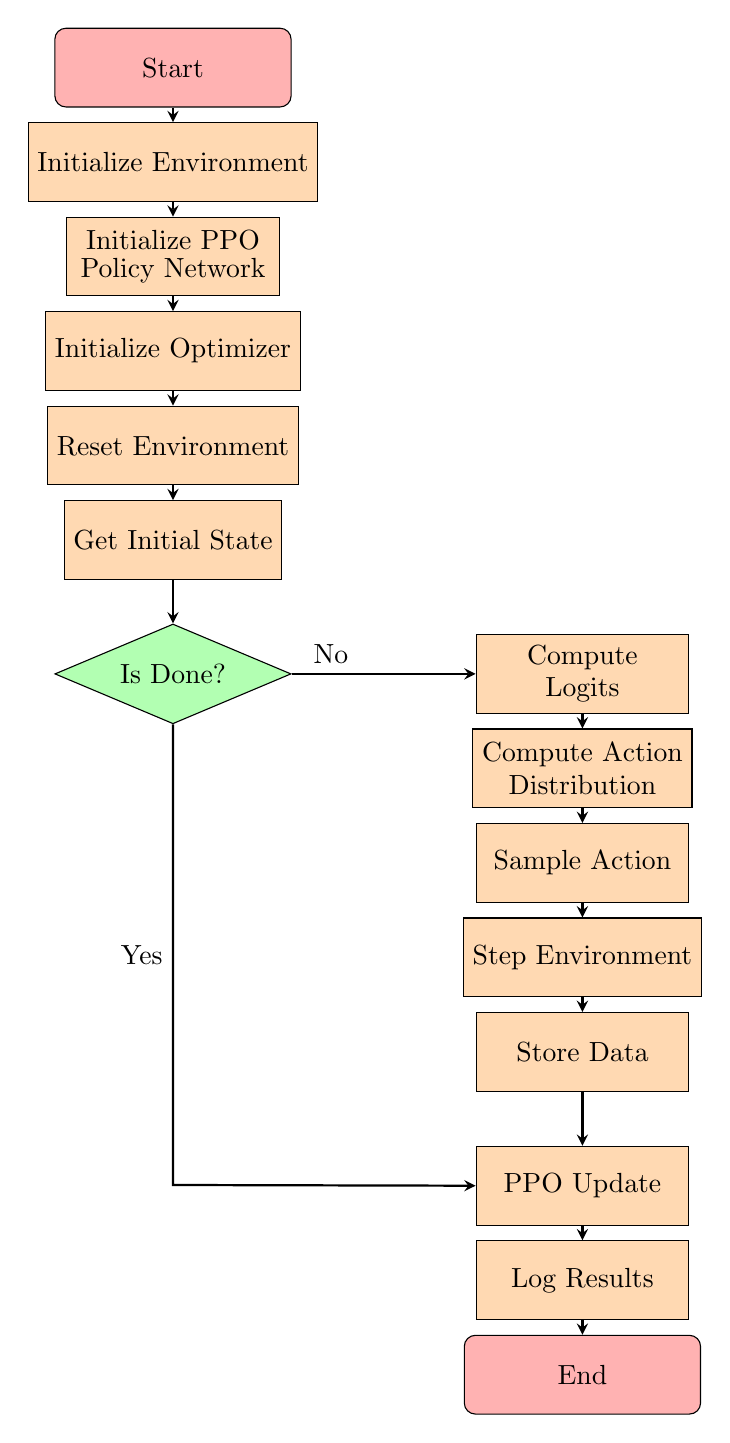
\begin{tikzpicture}[node distance=1.2cm]
    
    \node (start) [startstop] {Start};
    \node (initEnv) [process, below of=start] {Initialize Environment};
    \node (initNet) [process, below of=initEnv] {\shortstack{Initialize PPO \\ Policy Network}};
    \node (initOpt) [process, below of=initNet] {Initialize Optimizer};
    \node (resetEnv) [process, below of=initOpt] {Reset Environment};
    \node (getState) [process, below of=resetEnv] {Get Initial State};
    \node (doneCheck) [decision, below of=getState, yshift=-0.5cm, aspect=2] {Is Done?};
    
    \node (logits) [process, right of=doneCheck, xshift=4cm] {\shortstack{Compute \\ Logits}};
    \node (dist) [process, below of=logits] {\shortstack{Compute Action \\ Distribution}};
    \node (action) [process, below of=dist] {Sample Action};
    \node (envStep) [process, below of=action] {Step Environment};
    \node (storeData) [process, below of=envStep] {Store Data};
    
    \node (ppoUpdate) [process, below of=storeData, yshift=-0.5cm] {PPO Update};
    \node (logResults) [process, below of=ppoUpdate] {Log Results};
    \node (end) [startstop, below of=logResults] {End};
    
    \draw [arrow] (start) -- (initEnv);
    \draw [arrow] (initEnv) -- (initNet);
    \draw [arrow] (initNet) -- (initOpt);
    \draw [arrow] (initOpt) -- (resetEnv);
    \draw [arrow] (resetEnv) -- (getState);
    \draw [arrow] (getState) -- (doneCheck);
    
    \draw [arrow] (doneCheck.east) -- node[anchor=south] {No} ++(1,0) |- (logits.west);
    \draw [arrow] (logits) -- (dist);
    \draw [arrow] (dist) -- (action);
    \draw [arrow] (action) -- (envStep);
    \draw [arrow] (envStep) -- (storeData);
    \draw [arrow] (storeData) -- (ppoUpdate);
    \draw [arrow] (ppoUpdate) -- (logResults);
    \draw [arrow] (logResults) -- (end);
    
    \draw [arrow] (doneCheck.south) -- node[anchor=east] {Yes} ++(0,-5.85) -- (ppoUpdate.west);
    \end{tikzpicture} 
    \caption{PPO Policy Network Training Pipeline}
    \label{fig:policy_network}
\end{figure}

\par This architecture is designed to process the input features derived from market data and produce logits for the action probabilities. The logits indicate the likelihood of each possible action, where the actions are binary: 0 (no spoofing) and 1 (spoofing).

\par The initialization of the network weights is performed using the Kaiming Normal method for the weights of the linear layers, and biases are initialized to zero. The network is optimized using the Adam optimizer, with the learning rate set to $1 \times 10^{-3}$.

\par To optimize the policy network, we compute discounted rewards. Discounted rewards take into account future rewards to emphasize immediate actions that could indicate spoofing. The formula we used is:
\begin{equation}
R_t = r_t + \gamma R_{t+1}
\end{equation}
where $r_t$ is the reward at time step $t$ and $\gamma$ is the discount factor.

\par The Generalized Advantage Estimation (GAE) is used to compute more stable advantage estimates. The advantage $A_t$ at time step $t$ is calculated using:
\begin{equation}
A_t = \delta_t + \gamma \lambda A_{t+1}
\end{equation}

where $\delta_t = r_t + \gamma V(s_{t+1}) - V(s_t)$, and $V(s_t)$ represents the value function. This method smooths out the advantage estimates, making policy updates more stable and reliable; the detection of spoofing needs to be effective against the noisy and volatile nature of financial markets.

\par The PPO update mechanism is designed to adjust the network weights in a controlled manner. It calculates the loss function and performs gradient descent to update the policy. The loss function includes a clipped surrogate objective, a value function loss, and an entropy bonus. The clipped surrogate objective is defined as:
\begin{equation}
\begin{split}
L^{\text{CLIP}} = \mathbb{E} \Bigg[ &\min \Bigg( \frac{\pi_\theta(a_t|s_t)}{\pi_{\theta_{\text{old}}}(a_t|s_t)} \cdot A_t, \\
& \text{clip}\left(\frac{\pi_\theta(a_t|s_t)}{\pi_{\theta_{\text{old}}}(a_t|s_t)}, 1 - \epsilon, 1 + \epsilon \right) \cdot A_t \Bigg) \Bigg]
\end{split}
\end{equation}
where $\pi_\theta(a_t|s_t)$ represents the new policy, and $\pi_{\theta_{\text{old}}}(a_t|s_t)$ is the old policy.

\par The PPO update ensures that the policy improvement is conservative and stable when dealing with the highly dynamic and stochastic environment of financial markets. The inclusion of an entropy term in the loss function encourages exploration, preventing the policy from becoming too deterministic and potentially missing out on new strategies.

\section{Experimental Results}
\subsection{Hyperparameter Tuning}
\par The hyperparameter tuning process was divided into two phases. In the first phase, we compared the performance of the PPO model with and without rolling statistics in the anomaly score calculation to evaluate the impact of our feature engineering contribution. In the second phase, we focused on optimizing PPO parameters such as the learning rate, batch size, epochs, and spoofing threshold. Table \ref{tab:hyper_init} lists the feature weights used during anomaly detection.

\begin{table}[H]
    \centering
    \caption{Feature Weights for Anomaly Score Calculation}
    \label{tab:hyper_init}
    \begin{tabular}{|l|r|}
        \hline
        \textbf{Feature} & \textbf{Weight} \\
        \hline
        order\_flow\_imbalance & 0.15 \\
        cancel\_to\_received\_ratio & 0.15 \\
        price\_5\_std & 0.05 \\
        price\_10\_std & 0.05 \\
        price\_15\_std & 0.05 \\
        size\_5\_var & 0.05 \\
        size\_10\_var & 0.05 \\
        size\_15\_var & 0.05 \\
        spread & 0.10 \\
        last\_size\_5\_var & 0.05 \\
        last\_size\_10\_var & 0.05 \\
        hour\_of\_day & 0.15 \\
        hour\_15 & 0.05 \\
        hour\_16 & 0.05 \\
        hour\_17 & 0.05 \\
        hour\_18 & 0.05 \\
        hour\_19 & 0.05 \\
        \hline
    \end{tabular}
\end{table}

\par By removing our rolling statistics features, we heuristically adjusted the weight configuration as depicted in Table \ref{tab:hyper_adapt}.

\begin{table}[H]
    \centering
    \caption{Feature Weights for Anomaly Score Calculation without Rolling Statistics}
    \label{tab:hyper_adapt}
    \begin{tabular}{|l|r|}
        \hline
        \textbf{Feature} & \textbf{Weight} \\
        \hline
        order\_flow\_imbalance & 0.25 \\
        cancel\_to\_received\_ratio & 0.25 \\
        spread & 0.10 \\
        hour\_of\_day & 0.15 \\
        hour\_15 & 0.25 \\
        hour\_16 & 0.25 \\
        hour\_17 & 0.25 \\
        hour\_18 & 0.25 \\
        hour\_19 & 0.25 \\
        \hline
    \end{tabular}
\end{table}

\par These weights were selected based on domain knowledge and empirical experimentation. During hyperparameter tuning, we adjusted these weights to find the optimal combination that maximizes the model's performance.

\par The hyperparameters for the second phase of tuning are as follows:

\begin{enumerate}
\item{\textbf{Learning Rate:} This controls how much to change the model in response to the estimated error each time the model weights are updated.}

\[
\alpha \in \{1 \times 10^{-4}, 5 \times 10^{-4}, 1 \times 10^{-3}\}
\]

\item{\textbf{Batch Size:} Batch size influences the stability and speed of the training process. Smaller batch sizes typically provide a regularizing effect and lower generalization error, while larger batch sizes can speed up the training process.}

\[
\text{Batch Size} \in \{32, 64, 128\}
\]

\item{\textbf{Number of Epochs:} The number of epochs determines how many times the entire training dataset passes through the network. More epochs can lead to better learning, but may also cause overfitting if not controlled properly.}

\[
\text{Epochs} \in \{10, 20, 30\}
\]

\item{\textbf{Spoofing Threshold:} The spoofing threshold is unique to our application, defining the anomaly score threshold above which actions are classified as spoofing. We start with an initial value for our adaptive threshold.}

\[
\text{Spoofing Threshold} \in \{0.7, 0.8, 0.9\}
\]
\end{enumerate}

\par We empirically selected 10 of the most promising configurations that could potentially balance the trade-off between all the learning parameters. The hyperparameter tuning process leverages parallelization to efficiently explore the vast search space of the ten established hyperparameter configurations. Specifically, we employed the \texttt{joblib} library, which allows for parallel execution of all ten hyperparameter combinations across multiple CPU cores.

\subsection{Performance Analysis}

\par In terms of data splitting, we used 70\% of the data for training and 30\% for testing. Contiguous data segments were maintained to ensure the integrity of the time series and avoid cross-contamination between the datasets.

\textbf{Model Evaluation Metrics}:
    \begin{itemize}
        \item \textbf{Training Loss}: Combines actor and critic losses with an entropy term, guiding the optimization process. Lower loss indicates better performance.
        \item \textbf{Anomaly Scores}: Calculated based on predefined feature weights and market data features. Scores above the spoofing threshold indicate spoofing.
        \item \textbf{Cumulative Rewards}: Higher cumulative rewards indicate better policy performance in detecting spoofing and taking appropriate actions.
        \item \textbf{Reward Distribution}: Analyzes the effectiveness of the agent's actions, with positive rewards for correct spoofing detection and negative rewards for false positives.
    \end{itemize}

\textbf{Hypertuning Evaluation Metrics}:
    \begin{itemize}
        \item \textbf{Total Reward}: Sum of all rewards during the testing phase. Higher values indicate more effective spoofing detection.
        \item \textbf{Average Reward}: Mean value of rewards per step, indicating consistency and stability. Higher values suggest a more reliable model.
        \item \textbf{Standard Deviation of Rewards}: Measures reward variability. Lower values indicate more stable performance.
    \end{itemize}

\par The final results of our experiments are depicted in Figure \ref{fig:training_results}, including the anomaly scores over time, cumulative rewards over time, training loss over epochs, and reward distribution.

\par Before reaching these results, we performed hyperparameter tuning. The comparative analysis of the performance metrics of the model with and without rolling statistics is shown in Figure \ref{fig:hypertuning_results}. The anomaly detection phase and, by extension, the performance of the PPO model are significantly improved, as more subtle patterns in the data are captured. Cancellation ratio increased from 63\% to 89\%, which is closer to the 98.6\% cancellation records reported by Li, Polukarov, and Ventre (2023) \cite{Li_2023} in their statistical report. Training loss decreased from 0.24 to 0.13, and the maximum frequency of positive reward peaked at 20,000, compared to 17,000 without rolling statistics. This resulted in a 9,500 total reward, which is more than 125\% greater than the initial total reward.

\begin{figure}[H]
    \centering
    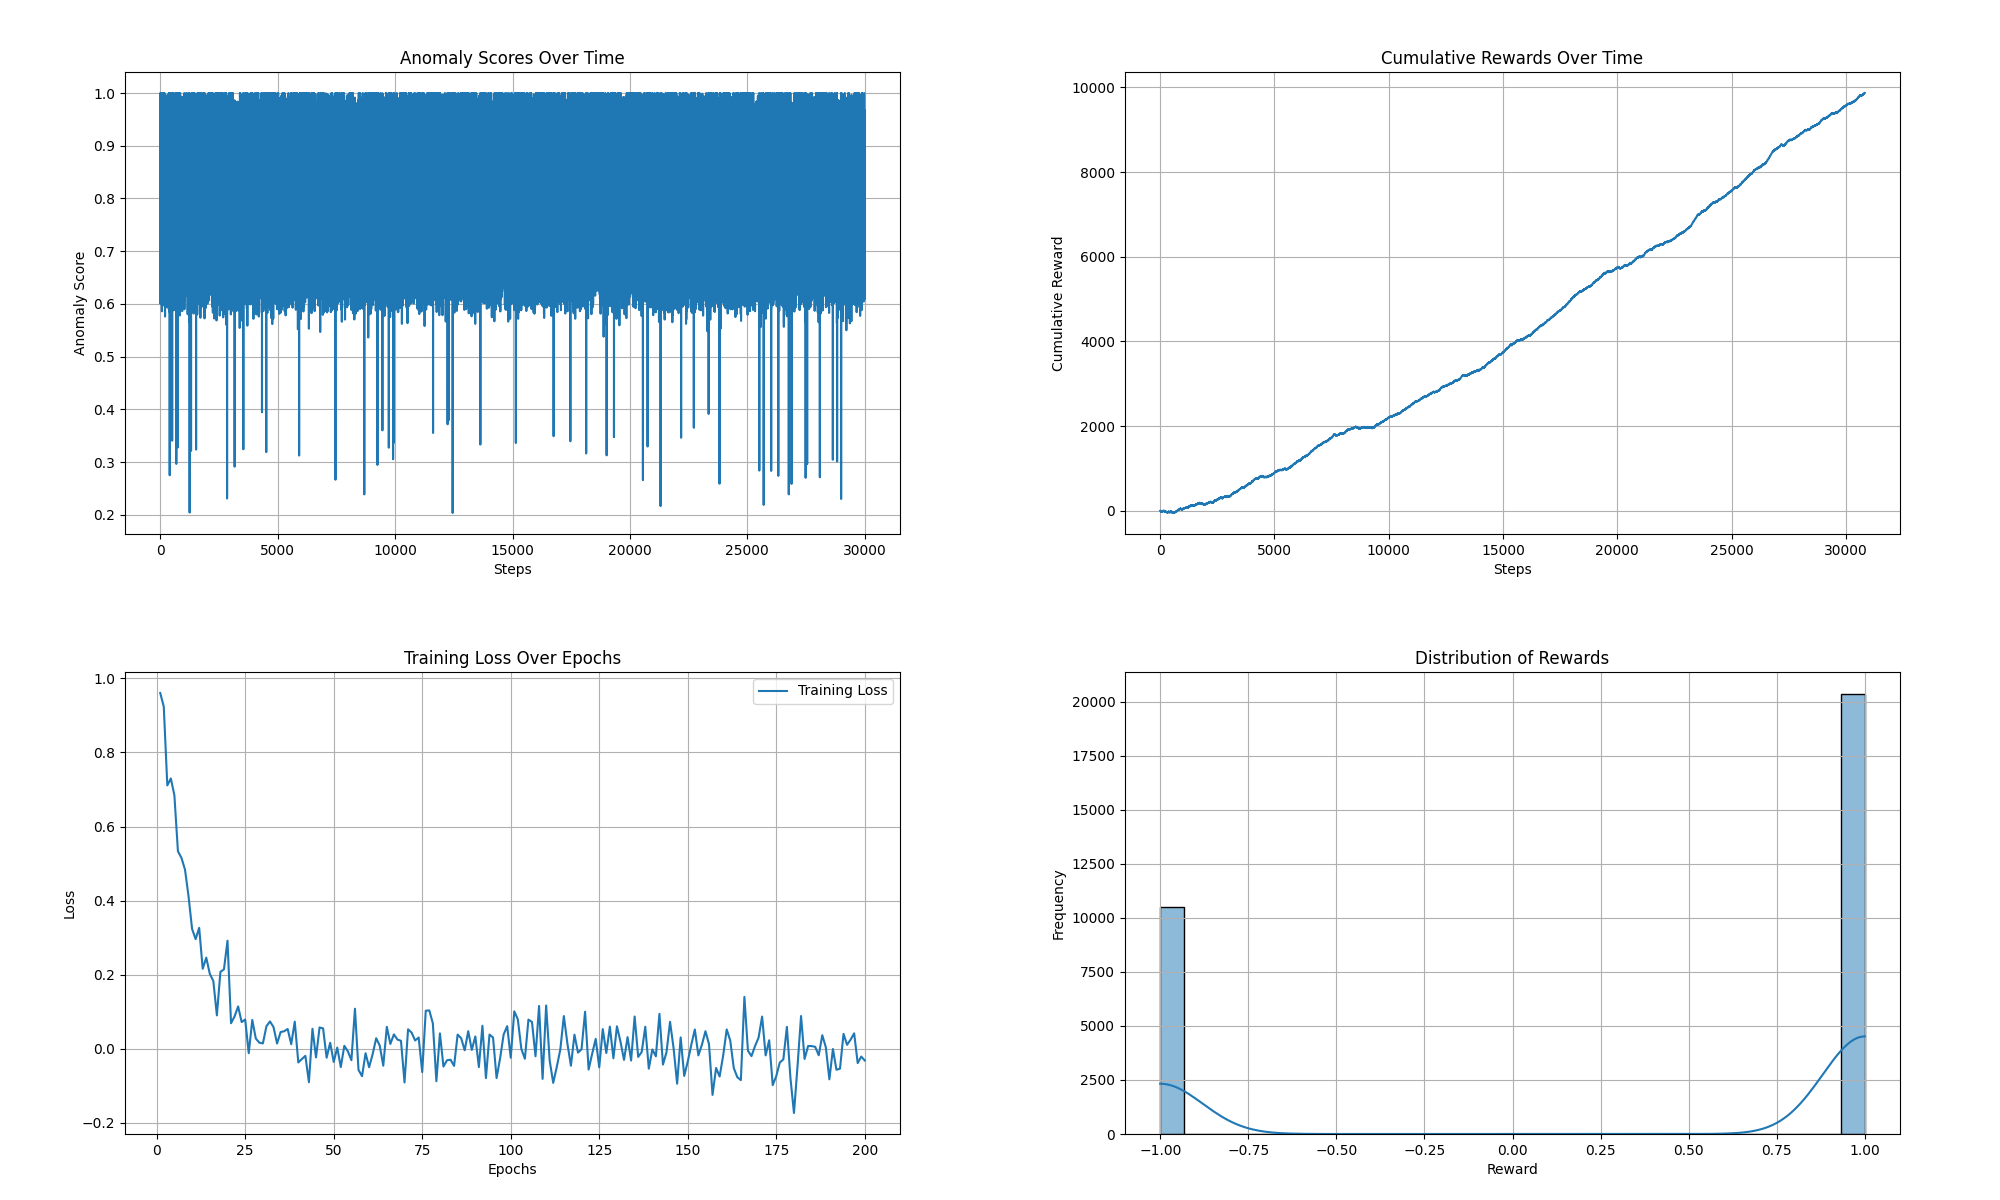
\includegraphics[scale=0.132]{./figures/training_results.png}
    \caption{Training results: Anomaly Scores Over Time (top left), Cumulative Rewards Over Time (top right), Training Loss Over Epochs (bottom left), Reward Distribution (bottom right).}
    \label{fig:training_results}
\end{figure}

\begin{figure}[H]
    \centering
    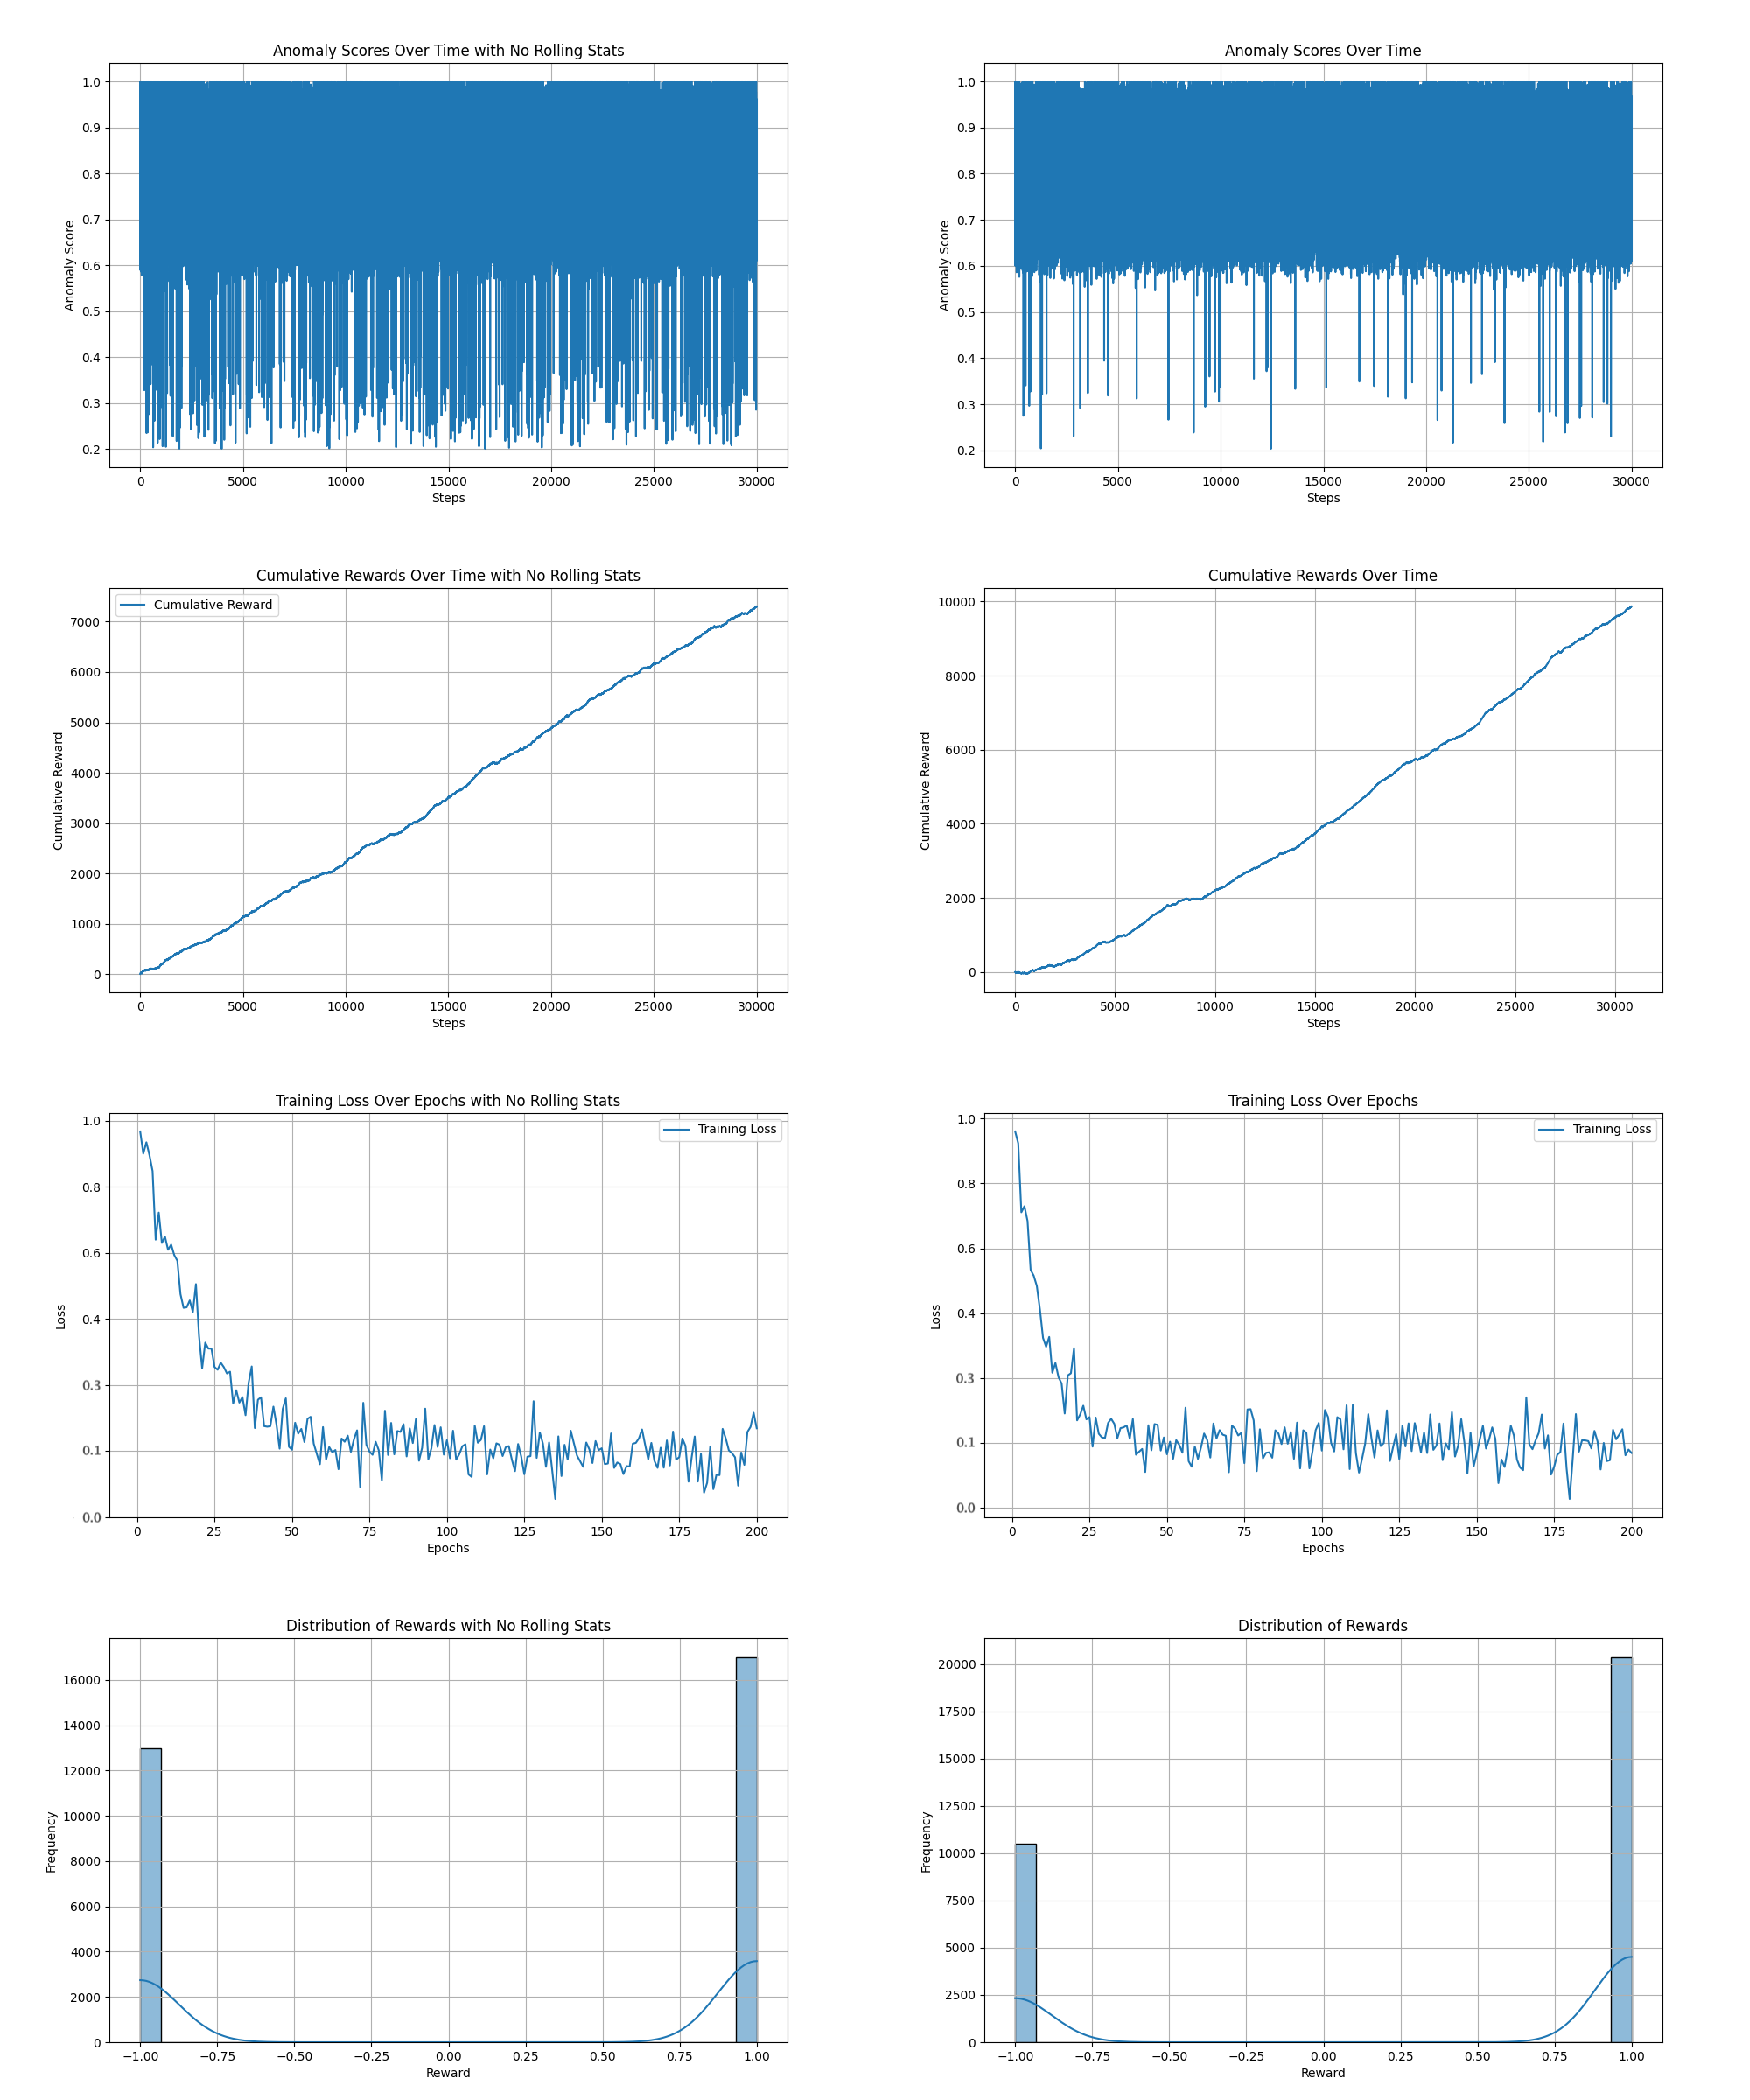
\includegraphics[scale=0.132]{./figures/hypertuning_results.png}
    \caption{Hypertuning results: Comparison of model performance without (left) and with rolling statistics (right).}
    \label{fig:hypertuning_results}
\end{figure}

\par For the second phase of hyperparameter tuning, focusing on the PPO parameters, we empirically selected 10 configurations based on their potential performance. Table \ref{tab:ppo_hyperparameters} provides a summary of these configurations along with their performance metrics, ranked by total reward.

\begin{table}[H]
\centering
\caption{Performance metrics for selected PPO configurations}
\label{tab:ppo_hyperparameters}
\renewcommand{\arraystretch}{1.5} % Increase row height
\begin{tabularx}{\columnwidth}{|>{\centering\arraybackslash}m{0.8cm}|>{\centering\arraybackslash}m{0.8cm}|>{\centering\arraybackslash}m{0.8cm}|>{\centering\arraybackslash}m{1.2cm}|>{\centering\arraybackslash}m{0.6cm}|>{\centering\arraybackslash}m{0.6cm}|>{\centering\arraybackslash}m{1cm}|}
\hline
\scriptsize \textbf{\makecell[c]{Total \\Reward}} & \scriptsize \textbf{\makecell[c]{Avg \\Reward}} & \scriptsize \textbf{\makecell[c]{Std \\Reward}} & \scriptsize \textbf{\makecell[c]{Learning \\Rate}} & \scriptsize \textbf{\makecell[c]{Batch \\Size}} & \scriptsize \textbf{\makecell[c]{Epochs}} & \scriptsize \textbf{\makecell[c]{Spoofing \\Threshold}} \\
\hline
9500         & 0.317      & 0.120       & $1 \times 10^{-3}$          & 128        & 30     & 0.8                 \\
9200         & 0.307      & 0.115       & $5 \times 10^{-4}$          & 128        & 30     & 0.8                 \\
9000         & 0.300      & 0.110      & $1 \times 10^{-3}$          & 64         & 20     & 0.8                 \\
8900         & 0.297      & 0.105       & $5 \times 10^{-4}$          & 32         & 20     & 0.8                 \\
8500         & 0.283      & 0.102       & $1 \times 10^{-3}$         & 128        & 30     & 0.7                 \\
8300         & 0.277      & 0.099       & $5 \times 10^{-4}$          & 32        & 20     & 0.9                 \\
8000         & 0.267      & 0.094       & $1 \times 10^{-3}$          & 64         & 20     & 0.7                 \\
7800         & 0.260      & 0.091      & $5 \times 10^{-4}$          & 64         & 20     & 0.7                 \\
7500         & 0.250      & 0.088      & $1 \times 10^{-4}$          & 32        & 10     & 0.8                 \\
7300         & 0.243      & 0.085      & $1 \times 10^{-4}$          & 64         & 10     & 0.9                 \\
\hline
\end{tabularx}
\end{table}

\par The results from above prove the feasibility of employing PPO in advancing market integrity, as the clear convergence of training loss over epochs (stabilizing around 0.13) indicates effective learning. Reward optimization managed to achieve consistent results, while minimizing volatility. However, it is clear that leveraging an unsupervised learning approach still represents a great challenge in accurately detecting legitimate spoof attempts. Only 89\% of orders were canceled, and, implicitly, can be marked as spoofed orders.

\par However, in our dataset, roughly 98.6\% open orders were eventually canceled. According to Li, Polukarov, and Ventre (2023) \cite{Li_2023}, \textit{"a total of 248,796 order submission and cancellation records were identified, with 233,134 occurring within the active area, 8,302 within the passive area, and 7,360 outside"}. This leads to 97\% of the order submissions and cancellations to occur within the active area, with only 3\% within the passive area \cite{Li_2023}.

\subsection{Discussion and Comparison}
\par Through our work, we managed to achieve all of our goals in terms of our contribution to the field of deep reinforcement learning in market surveillance. \textit{spoof.io}, the first available web tool for spoofing detection, has demonstrated the feasibility of employing PPO in detecting market manipulation. Additionally, our contribution to the feature engineering of rolling statistics of order price and size was proven to significantly improve the performance of our model. And lastly, we successfully harnessed Level 3 LOB information in processing time series as part of our model development.

\par After coming up with a good configuration as a result of carefully hypertuning both the anomaly detection features, and the PPO parameters, our model reached a great performance. With a clear convergence of training loss (stabilizing around 0.13) and accumulating a consistent total reward of 9,500 with minimal volatility, PPO has significant potential in enhancing market integrity.

\par A notable caveat of our work is the reliance on an anomaly detection model. One of our targets was developing a solution that can harness unlabeled data, without the obvious disadvantages of a supervised learning method. However, the amount of low-score orders, even after integrating an adaptive spoofing threshold, and performing hypertuning, denotes that there is still room for improvement. This conclusion comes from a comparison to the information on order cancellation in our dataset given by Li, Polukarov, and Ventre (2023) \cite{Li_2023}. This implies that a supervised approach could potentially yield more accurate and safer results. This is particularly critical given the safety and legal implications associated with detecting market manipulation. Ensuring the accuracy and reliability of detection systems is key to preventing false positives and the legal repercussions they might entail.

\par When compared to existing literature, our results show promising advancements. Previous studies have primarily focused on supervised learning approaches or unsupervised anomaly detection methods, such as those leveraging statistical physics and traditional machine learning techniques. Our PPO-based model, however, offers a deep reinforcement learning perspective, capable of dynamically adapting to market conditions in real-time and potentially uncovering more subtle forms of spoofing that other methods might miss.

\section{Conclusion}
\par In summary, our research demonstrates the potential of PPO in spoofing detection, offering a deep reinforcement learning approach that innovates and complements existing methodologies. 

\par Looking forward, several future research directions can be pursued to improve the efficacy of our agent. One significant area is the incorporation of online learning mechanisms, allowing the model to continually update and refine its detection capabilities with new data. This could involve the use of incremental learning techniques, allowing the model to adapt in real time as new trading data becomes available. Moreover, labeled datasets could be integrated. Advanced hyperparameter tuning methods, such as grid search or Bayesian optimization, could be implemented to systematically explore the hyperparameter space.

\par By addressing the highlighted limitations and exploring the suggested future directions, we can continue to enhance the reliability of \textit{spoof.io}, ultimately contributing to a fairer and more transparent trading environment.

\section*{Acknowledgment}
I would like to express my deepest gratitude to my supervisor, Lecturer Professor PhD Diana-Lucia Miholca, for her continuous guidance and support throughout this project.
I also extend my thanks to Haochen Li, Maria Polukarova, and Carmine Ventre for providing the dataset utilized in this research. Thanks to their exceptional results and insightful statistics as part of \cite{Li_2023}, our solution made use of the exact same L3 real market data on the LUNA/USD pair, gathered during the LUNA flash crash from May 2022. This research would not have been possible without their contribution.


\begin{thebibliography}{00}
\bibitem{Hendershott_Riordan_2013} T. Hendershott and R. Riordan, ``Algorithmic Trading and the Market for Liquidity,'' \textit{Journal of Financial and Quantitative Analysis}, vol. 48, no. 4, pp. 1001–1024, 2013, doi: 10.1017/S002210901
\bibitem{Armour_PFR} J. Armour, D. Awrey, P. Davies, L. Enriques, J. N. Gordon, C. Mayer, and J. Payne, ``181 Trading and Market Integrity,'' in \textit{Principles of Financial Regulation}, Oxford University Press, 2016, doi: 10.1093/acprof:oso/9780198786474.003.0009. [Online]. Available: https://doi.org/10.1093/acprof:oso/9780198786474.003.0009.
\bibitem{Dodd_Frank} ``Dodd-Frank Wall Street Reform and Consumer Protection Act,'' Pub. L. No. 111-203, 124 Stat. 1376, 2010. Available at U.S. Government Publishing Office: [https://www.govinfo.gov/content/pkg/PLAW-111publ203/pdf/PLAW-111publ203.pdf].
\bibitem{Li_2023} H. Li, M. Polukarova, and C. Ventre, ``Detecting Financial Market Manipulation with Statistical Physics Tools,'' arXiv preprint arXiv:2308.08683, 2023.
\bibitem{Tuc_2021} J.-N. Tuccella, P. Nadler, and O. Serban, ``Protecting Retail Investors from Order Book Spoofing using a GRU-based Detection Model,'' arXiv preprint arXiv:2110.03687, 2021.
\bibitem{Leang_2016} T. Leangarun, P. Tangamchit, and S. Thajchayapong, ``Stock price manipulation detection using a computational neural network model,'' in \textit{2016 Eighth International Conference on Advanced Computational Intelligence (ICACI)}, Chiang Mai, Thailand, 2016, pp. 337-341, doi: 10.1109/ICACI.2016.7449848.
\bibitem{Cao_2015} Y. Cao, Y. Li, S. Coleman, A. Belatreche, and T. M. McGinnity, ``Adaptive Hidden Markov Model With Anomaly States for Price Manipulation Detection,'' \textit{IEEE Transactions on Neural Networks and Learning Systems}, vol. 26, no. 2, pp. 318-330, Feb. 2015, doi: 10.1109/TNNLS.2014.2315042.
\bibitem{Lillo_2005} F. Lillo and J. D. Farmer, ``The key role of liquidity fluctuations in determining large price changes,'' \textit{Fluctuation and Noise Letters}, vol. 5, no. 2, pp. L209-L216, 2005, doi: 10.1142/S0219477505002574.
\bibitem{Yura_2014} Y. Yura, H. Takayasu, D. Sornette, and M. Takayasu, ``Financial Brownian Particle in the Layered Order-Book Fluid and Fluctuation-Dissipation Relations,'' \textit{Phys. Rev. Lett.}, vol. 112, no. 9, p. 098703, Mar. 2014, doi: 10.1103/PhysRevLett.112.098703.
\bibitem{Huyen_DMLS} C. Huyen, \textit{Designing Machine Learning Systems}, O'Reilly Media, Inc., 2022.
\bibitem{OpenAIPPO} OpenAI, ``OpenAI Baselines: PPO,'' 2017. [Online]. Available: https://openai.com/research/openai-baselines-ppo. Accessed: Apr. 1, 2024.
\bibitem{schulman2017proximal} J. Schulman, F. Wolski, P. Dhariwal, A. Radford, and O. Klimov, ``Proximal Policy Optimization Algorithms,'' arXiv preprint arXiv:1707.06347, 2017.
\bibitem{roderick2017implementing} M. Roderick, J. MacGlashan, and S. Tellex, ``Implementing the Deep Q-Network,'' arXiv preprint arXiv:1711.07478, 2017.
\bibitem{TRPO} J. Schulman, S. Levine, P. Abbeel, M. Jordan, and P. Moritz, ``Trust Region Policy Optimization,'' in \textit{Proceedings of the 32nd International Conference on Machine Learning}, vol. 37, F. Bach and D. Blei, Eds. Lille, France: PMLR, 2015, pp. 1889--1897. [Online]. Available: https://proceedings.mlr.press/v37/schulman15.html.
\bibitem{Montgomery_SMMLOB} J. D. Montgomery, ``Spoofing, Market Manipulation, and the Limit-Order Book,'' SSRN, May 2016. [Online]. Available: https://ssrn.com/abstract=2780579 or http://dx.doi.org/10.2139/ssrn.2780579.
\bibitem{Kularatnam2024} K. Kularatnam and M. Hayat, ``Detecting and Triaging Spoofing using Temporal Convolutional Networks,'' arXiv preprint arXiv:2403.13429, 2024, AAAI 2024 Workshop on AI in Finance for Social Impact. [Online]. Available: https://ar5iv.org/abs/2403.13429. Accessed: Jun. 3, 2024.
\end{thebibliography}

\end{document}
